\documentclass{jlreq}

\usepackage{amsmath}
\usepackage{array}
\usepackage{bm}
\usepackage{caption}
\usepackage{fancyhdr}
\usepackage{float}
\usepackage{graphicx}
\usepackage{listings}
\usepackage{multirow}
\usepackage{physics}
\usepackage{siunitx}
\usepackage{xcolor}

\lstset{
    language=Python, % 使用するプログラム言語を指定
    basicstyle=\ttfamily\footnotesize, % フォントの指定
    numbers=left, % 行番号を表示(必要な場合)
    numberstyle=\tiny, % 行番号のスタイル
    frame=single, % ソースコードを枠で囲む(必要な場合)
    breaklines=true, % 長い行を自動的に折り返す
    captionpos=b, % キャプションの位置を下にする
    showstringspaces=false, % 文字列内のスペースを表示しない
    keywordstyle=\color{blue}, % キーワードの色
    commentstyle=\color{green}, % コメントの色
    stringstyle=\color{red}, % 文字列の色
}
\renewcommand{\lstlistingname}{ソースコード}

\numberwithin{equation}{section}

\pagestyle{fancy}
\fancyhf{}
\fancyhead[R]{\thepage}

\begin{document}

\tableofcontents
\clearpage

\section{目的}
画像認識に必要な特徴抽出部を作成し,特徴評価を行うことで識別に必要な特徴の組み合わせを決める.

\section{実験手順}
\subsection{特徴抽出}
\begin{enumerate}
  \item 各画像に対して白黒反転と正規化を行った.
  \item 画素の縦方向・横方向の広がり方を捉えるために,重心,分散,ゆがみ,扁平度を縦横方向それぞれ求めて,8次元の特徴量抽出を行った.
  \item 特徴量の各次元のスケールを合わせるために標準化を行った.
  \item 正解数字と上記の8次元の特徴をカンマ区切りで並べた100行9列のcsvファイルを出力した.
\end{enumerate}

\subsection{特徴評価}
\begin{enumerate}
  \item クラス内分散とクラス間分散,およびそれらの比を求めるGoogle Colaboratoryのコードを実装し,
        識別に有効であると思われる2次元特徴の組み合わせを3つ求めた.
  \item 上記で求めた組み合わせについて,2次元散布図に出力するGoogle Colaboratoryのコードを実装し,識別に
        最も有効だと考えられる特徴の組み合わせを求めた.
\end{enumerate}

\section{結果}
\subsection{特徴抽出}
特徴抽出の実装をソースコード\ref{src:extract}に示す

\begin{lstlisting}[caption={特徴抽出の実装}, label=src:extract]
from os import fchdir
from google.colab import drive
drive.mount('/content/drive')

import matplotlib.pyplot as plt
# import pandas as pd
import numpy as np
from enum import Enum
import statistics
import csv

# PGM形式の画像を読み込む関数
def read_pgm(filename):
    with open(filename, 'rb') as f:
        # PGMファイルのヘッダーを読み込む
        header = f.readline().decode().strip()
        if header != 'P5':
            raise ValueError(f"Unsupported file format: {header}")

        # 画像サイズの読み込み
        size = f.readline().decode().strip()
        width, height = map(int, size.split())

        # 最大値の読み込み
        maxval = int(f.readline().decode().strip())

        # 画像データの読み込み
        im_data = f.read()  # バイナリデータを一度に読み込む

        # 画像配列に変換(リストを使う)
        im_array = []
        for i in range(height):
            row = []
            for j in range(width):
                pixel_value = im_data[i * width + j]
                row.append(pixel_value)
            im_array.append(row)

        return im_array, width, height

# 画素を反転する関数の定義
def rev_image(filename):
    # 画像を読み込む
    im_array, width, height = read_pgm(filename)

    # 反転処理(255から各画素値を引く)
    result = []
    for row in im_array:
        inverted_row = [255 - pixel for pixel in row]
        result.append(inverted_row)

    return result, width, height

# 画像を表示する関数
def show_image(im_array, width, height):
    plt.imshow(im_array, cmap='gray', aspect='auto')
    plt.axis('off')  # 軸を非表示にする
    plt.show()

# ==============================================================================
#                                  ここから自作
# ==============================================================================

FVALUE_SIZE = 8 # 特徴ベクトルのサイズ
TARGET_NUMBER_SIZE = 10 # 対象とする数字の種類数(0~9)
NUMBERS_LABEL_SIZE = 10 # それぞれの数字画像に対するラベル(候補)の数

# 特徴ベクトルの要素の添え字
# 重心
MUX = 0
MUY = 1
# 分散
VX = 2
VY = 3
# ゆがみ
SX = 4
SY = 5
# 扁平度
FX = 6
FY = 7

# 画素濃度正規化処理を行う関数
def normalize_image(im_rev, width, height):
    # 分母の算出
    denominator = 0
    for y in range(height):
      for x in range(width):
        denominator += im_rev[y][x]

    # 正規化処理
    result = []
    for y in range(height):
      row = []
      for x in range(width):
        normalized = im_rev[y][x]/denominator
        row.append(normalized)
      result.append(row)

    return result, width, height

# 重心を求める関数
def get_center(im_norm, width, height):
    ux = uy = 0
    for y in range(height):
      for x in range(width):
        ux += (x + 1) * im_norm[y][x]
        uy += (y + 1) * im_norm[y][x]

    return ux, uy

# 分散を求める関数
def get_variance(im_norm, width, height, ux, uy):
    vx = vy = 0
    for y in range(height):
      for x in range(width):
        vx += im_norm[y][x] * (x + 1 - ux) ** 2
        vy += im_norm[y][x] * (y + 1 - uy) ** 2

    return vx, vy

# ゆがみを求める関数
def get_skewness(im_norm, width, height, ux, uy, vx, vy):
    sx = sy = 0
    for y in range(height):
      for x in range(width):
        sx += im_norm[y][x] * (x + 1 - ux) ** 3
        sy += im_norm[y][x] * (y + 1 - uy) ** 3
    sx /= pow(vx, 1.5)
    sy /= pow(vy, 1.5)
    return sx, sy

# 扁平度を求める関数
def get_flatness(im_norm, width, height, ux, uy, vx, vy):
    fx = fy = 0
    for y in range(height):
      for x in range(width):
        fx += im_norm[y][x] * (x + 1 - ux) ** 4
        fy += im_norm[y][x] * (y + 1 - uy) ** 4

    fx /= pow(vx, 2)
    fy /= pow(vy, 2)
    return fx, fy

# 特徴抽出を行う関数
def extract_features_without_normalization(filename):
    # 画像を反転
    im, width, height = rev_image(filename)
    # 画像の正規化
    im, width, height = normalize_image(im, width, height)

    # 特徴量の算出
    fvalue = [0] * FVALUE_SIZE
    fvalue[MUX], fvalue[MUY] = get_center(im, width, height)
    fvalue[VX], fvalue[VY] = get_variance(im, width, height, fvalue[MUX], fvalue[MUY])
    fvalue[SX], fvalue[SY] = get_skewness(im, width, height, fvalue[MUX], fvalue[MUY], fvalue[VX], fvalue[VY])
    fvalue[FX], fvalue[FY] = get_flatness(im, width, height, fvalue[MUX], fvalue[MUY], fvalue[VX], fvalue[VY])

    return fvalue

# 特徴量の標準化をする関数
# fvalues_t: ある次元についての全画像の特徴量をまとめたベクトル
def standardize_feature_value(fvalues_t):
    for fvalue_t in fvalues_t:
      # 平均値の算出
      ave = statistics.mean(fvalue_t)
      print('ave = %f' % ave)
      # 標準偏差の算出
      sd = statistics.pstdev(fvalue_t)
      print('sd = %f' % sd)
      # 標準化
      for i in range(len(fvalue_t)):
        fvalue_t[i] = (fvalue_t[i] - ave) / sd

    return fvalues_t.T.tolist()

# 全画像の特徴量を計算し,CSVファイルとして出力する関数
def make_features_csv(dataset_path):
    fvalues = []
    # CSVファイルの作成
    with open('/content/drive/MyDrive/pattern/week01/feature.csv', 'w') as f:
      writer = csv.writer(f)

      # 各画像から特徴量を算出して2次元配列にまとめる
      for i in range(TARGET_NUMBER_SIZE):
        for j in range(NUMBERS_LABEL_SIZE):
          filename = f'{dataset_path}number{i}_{j}.pgm'
          # 特徴抽出部
          row = extract_features_without_normalization(filename)
          fvalues.append(row)

      # 特徴量の標準化
      fvalues_t = np.array(fvalues).T
      fvalues = standardize_feature_value(fvalues_t)

      # ラベルの追加
      for i in range(TARGET_NUMBER_SIZE):
        for j in range(NUMBERS_LABEL_SIZE):
          fvalues[i * TARGET_NUMBER_SIZE + j] = [i] + fvalues[i * TARGET_NUMBER_SIZE + j]

      # CSVへの書き込み
      writer.writerows(fvalues)

# ==============================================================================
#                                   実行部分
# ==============================================================================

dataset_path = '/content/drive/MyDrive/pattern/sample_data/number/'
make_features_csv(dataset_path)
\end{lstlisting}

また,CSVの出力結果を表\ref{tab:csv}に示す.

\begin{table}[H]
  \centering
  \caption{特徴量をまとめたCSVファイル}
  \scalebox{0.4}{\begin{tabular}{|r|r|r|r|r|r|r|r|r|}
      \hline
      0 & -0.7505019636430198   & 1.6188340268031158    & 1.7195994199875546   & -0.20294393081950754 & 0.564766303576569     & -0.7395120211897082   & -0.6966344793270051   & -0.4103744830005732   \\ \hline
      0 & -1.6858765577628123   & 1.6765347175175025    & 1.7667123102537383   & -0.20288770510755738 & 0.6438224332723195    & -0.7505844059340022   & -0.6849688719804399   & -0.4004040011881824   \\ \hline
      0 & -0.5991783413667354   & 0.24199446512870923   & 1.619255613667175    & -0.557535809445395   & 0.5674972061973432    & 0.2937959251580505    & -0.7311369964924413   & 0.019070298375090527  \\ \hline
      0 & -1.4783996303652014   & 0.238095713508989     & 1.620668466979348    & -0.44185008941780723 & 0.5796615334306591    & 0.4560611406914342    & -0.7094259791897896   & -0.012562040030783102 \\ \hline
      0 & -0.547417308148819    & 0.18049153944985816   & 1.6529559779934184   & -0.26160676249904125 & 0.5025642834279817    & -0.7356992361360449   & -0.6684977597246927   & -0.16240037745468014  \\ \hline
      0 & -1.4225462752635991   & 0.2525412501756195    & 1.7561796245708452   & -0.3035449180770797  & 0.5845235214707181    & -0.7801548944092326   & -0.6443913655212371   & -0.3180086977333264   \\ \hline
      0 & -0.3055376846544883   & -0.7471983482725616   & 1.6347499226168196   & -0.7167465281441867  & 0.3372565006863208    & 0.5226149241057306    & -0.7224605916449677   & 0.18311612678312153   \\ \hline
      0 & -1.1374776196629608   & -0.5602300463662574   & 1.7100068441161496   & -0.4834042989175053  & 0.29485621071785484   & 0.5796368946665174    & -0.5115069687808594   & 0.29291474449897376   \\ \hline
      0 & 0.32957041777683865   & -1.0596832021463698   & 1.723984778565471    & -0.27256696481840414 & 0.5645378584673366    & -0.68742346067483     & -0.700453716684531    & -0.35764928735397167  \\ \hline
      0 & -0.49674294970133953  & -0.9951264913720118   & 1.710127029351941    & -0.14125097642342002 & 0.5670059285188777    & -0.7822842393436301   & -0.6550793318285427   & -0.406865990488131    \\ \hline
      1 & -1.1502944111727695   & 1.9234784615981662    & -1.89756712803103    & 1.2845886875821695   & -1.0946552381457193   & -0.8613129426982848   & 0.6831412280080215    & -1.3629550178846375   \\ \hline
      1 & -0.4119977724061121   & 1.945370434555909     & -1.9782605566173856  & 1.3638753647153539   & -0.6772305901097941   & -0.7289710443691599   & 0.7797882241806021    & -1.3619595253769399   \\ \hline
      1 & -0.9974503200874595   & 0.3726032046977007    & -1.9932904998872114  & 0.9184354801222621   & -1.2174112702125024   & 0.6814714295596438    & 1.2277597648161631    & -0.9255594390113008   \\ \hline
      1 & -0.3783519630111141   & 0.5410696776159609    & -2.06621516405939    & 1.2124205941318025   & -0.9688338687838614   & 0.4558805911738451    & 0.6672687201719257    & -1.1795818490926688   \\ \hline
      1 & -0.8398976517574681   & 0.4076270969540033    & -1.9381117602059268  & 1.308082047563426    & -1.0482335296596454   & -0.7603679664811493   & 0.7416902161444016    & -1.3712541451407423   \\ \hline
      1 & -0.15197440905607076  & 0.4919847263578375    & -1.993108285429878   & 1.2501437702481466   & -0.763886673560609    & -0.730099699878351    & 1.471040099522346     & -1.343031294807703    \\ \hline
      1 & -1.052008274340966    & -0.5559678043691952   & -2.0882299964577262  & 0.8679827250095452   & -1.3592933473132667   & 0.7316772159768109    & 0.7304931940674996    & -0.9464980981973647   \\ \hline
      1 & -0.32497857483292575  & -0.32943469437858586  & -2.0416483383983373  & 1.0649026789146483   & -2.626505044696921    & 0.4118598187017524    & 4.5174237061730365    & -1.1797464491373513   \\ \hline
      1 & -0.045359958357559196 & -0.7589838372400106   & -1.852710424229122   & 1.4053931415934149   & -0.8598150621017918   & -0.7988574766028008   & 0.7132958216579969    & -1.3713848490785634   \\ \hline
      1 & 0.6918701609192895    & -0.6985984420079137   & -1.9291063079998405  & 1.4997309990401726   & -0.8245855347724482   & -1.0260787955753505   & 1.8723911121116616    & -1.108168260723057    \\ \hline
      2 & 0.2815750880673933    & 1.4864964284908084    & 0.2850634489807806   & 1.7443928869186907   & -0.015039947965738952 & 0.005113332245970757  & -0.4119897926537303   & -1.4812519020539003   \\ \hline
      2 & -0.3150219610108596   & 1.6617828707625644    & 0.3303010400973673   & 1.7921611144419949   & -0.08535802506694906  & -0.017986997553344763 & -0.3950123800894682   & -1.468743584102489    \\ \hline
      2 & 0.8843805836376064    & -0.10804644108959344  & 0.2995722543503759   & 1.0125356908083727   & -0.49008752230276076  & 1.7088915266444342    & -0.41590846457757985  & -0.4908322639389306   \\ \hline
      2 & 0.22613333450365813   & 0.280964911288965     & 0.2683020973062472   & 1.3226232166118406   & -0.3995372701268181   & 1.0923345289354989    & -0.4313554857565739   & -1.0176463671945997   \\ \hline
      2 & 0.7107114178533728    & 0.06028929784232804   & 0.26994999444782947  & 1.6809521485024992   & -0.11248081125720324  & -0.01654932567850504  & -0.4158474212243854   & -1.4543362292306279   \\ \hline
      2 & -0.15351217624875754  & 0.23385038088959337   & 0.29926015403240835  & 1.6947694803622675   & 0.0009677591272742021 & -0.11001948210023349  & -0.4141609520438707   & -1.4802630126846665   \\ \hline
      2 & 0.9145006857321641    & -1.015932271126223    & 0.2854162784172602   & 1.025979060881825    & -0.49517909629966034  & 2.1637652254228965    & -0.45824218413569034  & 0.8517680511931696    \\ \hline
      2 & 0.3456545674086915    & -0.8132386191838791   & 0.308612624293259    & 1.0309120682504267   & -0.4361113813742956   & 1.6247635955056183    & -0.42895476194505966  & -0.5914765210110531   \\ \hline
      2 & 1.2818796444623342    & -1.1479481121255817   & 0.2796469595731348   & 1.7466164979788041   & -0.017356680666722347 & -0.07610108355643715  & -0.4243972274865082   & -1.4906421401132828   \\ \hline
      2 & 0.6791010432703759    & -1.0177914219883109   & 0.33350247564408886  & 1.7930547497593032   & 0.25017899334599936   & -0.007835878406110535 & 0.0028608653461752484 & -1.4518645395387986   \\ \hline
      3 & 0.4324087772043067    & 1.6162155361203323    & -0.24698612773404097 & 0.9722562106386333   & -1.3995894421623583   & -0.6058295989338163   & -0.1118950471226377   & -1.074577392081721    \\ \hline
      3 & 2.2520121082679223    & 1.6881477182522464    & -0.15482369023495818 & 1.0429849559672255   & -1.2853604407338712   & -0.499957084108876    & -0.12041864281398215  & -1.038886355919687    \\ \hline
      3 & 0.6384522350839018    & 0.11731066850202038   & -0.4288221754026614  & 0.45930940276575744  & -1.466091219845665    & 0.7482648351413351    & -0.049707261802942215 & -0.4660367891712773   \\ \hline
      3 & 2.4294638355697433    & 0.37975634871058955   & -0.4344525245269182  & 0.6138917908141878   & -1.4111187413633923   & 0.5122595118124926    & -0.06673543646537364  & -0.5969061709918896   \\ \hline
      3 & 0.6280712346376192    & 0.10087997912165002   & -0.22703537047695466 & 0.8809237031155397   & -1.3474459722698697   & -0.5633327884831543   & -0.13252107426520435  & -1.0244360601112958   \\ \hline
      3 & 2.3256719012480995    & 0.25193787128177125   & -0.19765565741856678 & 0.919066359930807    & -1.306688496577964    & -0.41837544955249023  & -0.13562245255057062  & -1.018053047538716    \\ \hline
      3 & 0.6692118293642877    & -0.839220317287287    & -0.347913805761593   & 0.45623149327595336  & -2.0440231379163887   & 1.267167232531805     & 0.7006216356228862    & 0.973032935625555     \\ \hline
      3 & 2.2889219829666363    & -0.6062542592791854   & -0.5047964431580446  & 0.4377208120344912   & -1.4409590431024388   & 0.7732873912887444    & -0.08440051250374143  & -0.4376707632711242   \\ \hline
      3 & 1.446783353644286     & -1.0958185598366779   & -0.28366144453424547 & 1.0010763286438578   & -1.3872388859410745   & -0.5816326011632458   & -0.12464621299677496  & -0.9135460098981791   \\ \hline
      3 & 3.1999739519345436    & -0.9628919025187859   & -0.0868546068662222  & 1.0188693668272775   & -1.2589179877996126   & -0.5148419902016088   & -0.12211854111849461  & -1.0612249311854123   \\ \hline
      4 & -0.08996876009586084  & 1.5156617847809382    & -0.6843301309241576  & -1.7025132311950875  & -1.1863237593522473   & -1.3933275285254592   & 0.15990551046390877   & 1.1020843275373475    \\ \hline
      4 & 0.5549348634054816    & 1.6901491943032878    & -0.7019032327579995  & -1.671855902696148   & -1.2273652973934135   & -1.4588935806564922   & 0.18615595998536205   & 1.3640343977053837    \\ \hline
      4 & -0.03350537524022351  & 0.21729677370651004   & -0.8568904970078747  & -2.033288996715898   & -1.2577778975161844   & -0.869400256392182    & 0.22276661176619905   & 1.579582292755197     \\ \hline
      4 & 0.5335159603996708    & 0.4554336787371825    & -0.757133100896808   & -1.9987970274975442  & -0.8333662846265714   & -0.7806079325968148   & 0.5425738860086755    & 1.5369582135756854    \\ \hline
      4 & 0.21288013099913677   & 0.050041127639290715  & -0.7761733157389811  & -1.763612995569397   & -1.1244603680233272   & -1.3490799746453537   & 0.21999679935092886   & 1.087744705034366     \\ \hline
      4 & 0.677119780759799     & 0.23431363082853282   & -0.7353682450115624  & -1.7295584674198792  & -1.0427076699911895   & -1.331860578250284    & 0.21077505849447342   & 1.0433870664175287    \\ \hline
      4 & -0.022098238928653854 & -0.6840790638684932   & -0.976732877369972   & -2.1073697921508083  & -1.2762679037486209   & -0.7277353737643335   & 0.12840212322071587   & 1.2783257343365415    \\ \hline
      4 & 0.4187525230965226    & -0.5282631827660336   & -0.8979116598826082  & -2.050844926339701   & -1.1993734523809911   & -0.49403023930044954  & 0.29338759823536326   & 1.2982873816714031    \\ \hline
      4 & 1.0323719380173049    & -1.133720071483921    & -0.7934787986832729  & -1.6911790913698617  & -1.1714054518334829   & -1.4252441612122781   & 0.15828925889568976   & 1.051838465183481     \\ \hline
      4 & 1.4624557683230377    & -0.9906138967171265   & -0.7426327364009196  & -1.7017656714661102  & -1.1521089129765074   & -1.3864653956445798   & 0.14153083470093203   & 1.0761910396167258    \\ \hline
      5 & -1.1458540675067985   & 1.511112758535061     & 0.2849035994210112   & 0.6636262059674971   & 0.9018751148340941    & -0.8497637218093493   & -0.5187300777812218   & -0.45654597641716915  \\ \hline
      5 & 0.11505644873003557   & 1.7900799789923372    & 0.1964166221466978   & 0.6699508466593965   & 0.9862471381338136    & -0.9078410129126707   & -0.49072116830899787  & -0.19066364755731297  \\ \hline
      5 & -1.2356054260388054   & 0.15331530010990585   & -0.04306074012893348 & 0.10341018064667722  & 1.2553891722995214    & 0.17557272866943305   & -0.4655062802175852   & 0.1538648712620504    \\ \hline
      5 & 0.14883297458265382   & 0.39476205343814774   & 0.3897135078798446   & 0.15871591823054665  & -0.5101902199765361   & 0.13776294185335988   & 2.052991523815105     & 0.055432956490240375  \\ \hline
      5 & -0.948721214056287    & 0.09828889125830197   & 0.2845420541204779   & 0.5281539505631333   & 0.954776174813829     & -0.8322909820876497   & -0.5238541409790956   & -0.38448502739307566  \\ \hline
      5 & 0.12288585796173733   & 0.2504077732773677    & 0.2471896126063867   & 0.5811838426262875   & 1.0538934183457653    & -0.6979657468856478   & -0.5062405371882471   & -0.41053931836682683  \\ \hline
      5 & -1.1927789534302309   & -0.7273740639197056   & 0.06878585327753672  & 0.06089801109039842  & 1.1874883344914207    & 0.21607067498195573   & -0.5330134331652924   & 0.08858016424662787   \\ \hline
      5 & 0.03113974813098458   & -0.5856248242855696   & 0.057810057845543876 & 0.023509881840044135 & 1.126648012086324     & 0.3226795436503074    & -0.5387634285845406   & 0.15535206991810302   \\ \hline
      5 & -0.12173221756445515  & -1.100634837994781    & 0.2925966483804718   & 0.6626611203158304   & 0.9463896654778619    & -0.9559183256966027   & -0.5028497792112671   & -0.41498781300939086  \\ \hline
      5 & 1.2211805618909914    & -0.927799800112852    & 0.11434140856231549  & 0.6789020473482109   & 1.0264624165210403    & -0.7589976187784101   & -0.5074267378632933   & -0.3870256671400641   \\ \hline
      6 & -1.7928969660054768   & 1.7476346159115212    & 0.4058005619098969   & -0.5789812040952772  & 0.7271493337080762    & -1.1516837625790697   & -0.5329070874297799   & 0.5244357803627048    \\ \hline
      6 & -0.3239232125582289   & 1.935299185898393     & 0.39592686818603634  & -0.611996694049259   & 0.6962045669964       & -1.1306363016740417   & -0.5453287603740696   & 0.5484769003388755    \\ \hline
      6 & -1.5553841659551668   & 0.4067332209513329    & 0.1755769514797933   & -0.9491138263639589  & 0.661601986613641     & -0.18251979382990047  & -0.5478942925979682   & 0.9714305788485464    \\ \hline
      6 & -0.21143620824621512  & 0.6596963050167146    & 0.3208128084945173   & -0.9955873494258015  & 0.8025977534559208    & -0.3029132687345836   & -0.3784967569964706   & 1.002193980827798     \\ \hline
      6 & -1.6136219075224134   & 0.2691208787729008    & 0.4359315824249425   & -0.6588543830397865  & 0.7528336046274684    & -1.1085391662265072   & -0.5542126370337189   & 0.4913503170092743    \\ \hline
      6 & -0.40113680382375483  & 0.5022231284106857    & 0.4214785583675088   & -0.6702605603214506  & 0.7796681669468988    & -1.1041817218531034   & -0.554520098153377    & 0.49983376097849075   \\ \hline
      6 & -1.683592076870002    & -0.5548734627356846   & 0.10972479785579377  & -1.0008949725904428  & 0.7747325028221945    & -0.015002900347127857 & -0.531015760201802    & 1.0050346403630026    \\ \hline
      6 & -0.4457875708297378   & -0.3297597016842247   & 0.2458006328355942   & -1.0769031175491879  & 0.7057981321770266    & -0.06816751332298104  & -0.5535959565671046   & 1.0438803688828477    \\ \hline
      6 & -0.7184343625075855   & -0.9194560859016928   & 0.3830432847578705   & -0.5501075000384257  & 0.7147040702334604    & -1.0689403714780212   & -0.5547740864499925   & 0.43424217215575306   \\ \hline
      6 & 0.6987294021981362    & -0.7891778220006406   & 0.42558707952982344  & -0.5573483919978821  & 0.7858147643052159    & -0.9721505129744046   & -0.4783433258475188   & 0.48175756068595615   \\ \hline
      7 & -0.8935175737100766   & 0.41323406458540335   & -0.977265979482646   & 0.584214633420661    & 0.5729133739977754    & 1.3554594692565578    & 0.34989714204831907   & -0.4035231386558744   \\ \hline
      7 & -0.09438306061474465  & 0.5067194524079796    & -0.9578166666589226  & 0.4898031429364303   & 0.4186677938035579    & 1.5814076105425183    & 0.3371295462121943    & -0.20070060970353107  \\ \hline
      7 & -0.43232681844226906  & -1.0709241299952224   & -0.8923196810934674  & -0.2655896576251234  & -0.004124848540627453 & 2.7660041772864123    & 0.19879631782988866   & 1.0544316382278054    \\ \hline
      7 & 0.20819973775986325   & -0.7104412157020116   & -0.9871273398996971  & -0.07882103456210283 & -0.6346007635538771   & 2.430467954535985     & 1.469199008086529     & 0.9988556390644544    \\ \hline
      7 & -0.5216151728608147   & -0.8972085561304999   & -0.688466793584815   & 0.5338126562472598   & 4.3154051739206105    & 1.2009896184217268    & 6.443260649755727     & -0.37701360221729474  \\ \hline
      7 & 0.009068828499826388  & -0.7505710157073063   & -1.0587799681938277  & 0.5748219574518014   & 0.7052330734417755    & 1.2288560969624387    & 0.3263545829685227    & -0.4438680576397753   \\ \hline
      7 & -0.09107825303991968  & -1.944310619720719    & -0.9337021962902002  & -0.48079793784278246 & 0.03826093705628474   & 2.85135224115267      & 0.19898649181859085   & 1.274696060434248     \\ \hline
      7 & 0.3566469994356704    & -1.579081392528893    & -1.0067314829266891  & -0.22951295139118263 & 0.2571993627519306    & 2.2836394824040074    & 0.2660690093835922    & 0.5960352415169743    \\ \hline
      7 & 0.2785455852273237    & -2.2840959751290764   & -1.0919906729360205  & 0.5514514984156789   & 0.5096849873006177    & 1.4762814850670625    & 0.30516553363363574   & -0.32896368107925966  \\ \hline
      7 & 0.9963812134062597    & -2.1068309915611936   & -1.1229039228899251  & 0.5731435596754463   & 1.180368049896408     & 1.4553123140671165    & 1.4064084617151584    & -0.266848830086008    \\ \hline
      8 & -1.8499216462591515   & 1.558927076035382     & 0.7128829499297484   & -0.24026259003544495 & 0.5950054358022249    & -0.5896608113725799   & -0.5622957844330302   & -0.27377062636529237  \\ \hline
      8 & 0.5885622158916985    & 1.8276703064912339    & 0.693400729667256    & -0.2889765833289639  & 0.6005907337856888    & -0.5899924760243772   & -0.5583166410913445   & -0.29949036870131246  \\ \hline
      8 & -1.7169590641019767   & 0.26985700007422964   & 0.49938342749057574  & -0.6003668167183656  & 0.6892039930548387    & 0.27126769241270293   & -0.5750238010468831   & 0.07432594635637894   \\ \hline
      8 & 0.5956041914307484    & 0.5510501783777668    & 0.5464749119331737   & -0.5850382008991518  & 0.45408929860459274   & 0.10874117999314428   & -0.2401485597626585   & 0.22108915129797768   \\ \hline
      8 & -1.6792876148649494   & 0.18463120997872207   & 0.7669716528665389   & -0.32186578332892274 & 0.6822385395249442    & -0.6978108755614705   & -0.5589508688701588   & -0.31692674852970854  \\ \hline
      8 & 0.6586744819324127    & 0.4024593955624164    & 0.6612642089823941   & -0.2718281215178707  & 0.6627454657142003    & -0.722476361919405    & -0.5699994390686948   & -0.29473027679200714  \\ \hline
      8 & -1.5914234386090869   & -0.5707926087445433   & 0.47531554157969597  & -0.654559823309262   & 0.5924882221484513    & 0.3790438713339161    & -0.5796407529573431   & 0.17029132533147923   \\ \hline
      8 & 0.7079655067005772    & -0.4376118121863158   & 0.507970259423671    & -0.6654164755797091  & 0.5314018401963387    & 0.38443620804644624   & -0.5815310060942634   & 0.16890337544792466   \\ \hline
      8 & -0.8337937855932361   & -1.053507216984442    & 0.684609862689906    & -0.22045658651533667 & 0.6068164938900702    & -0.7453029156278262   & -0.5661373109472586   & -0.29540144916089045  \\ \hline
      8 & 1.5324179829135964    & -0.8731596501818796   & 0.5529978758185914   & -0.1538831806996769  & 0.5964508066567646    & -0.6736468365915298   & -0.5905162122415345   & -0.3171706103336712   \\ \hline
      9 & -0.22009592257040683  & 1.3909946501971604    & 0.8274968453559435   & -0.6274017757446504  & 0.09980935508216103   & 0.13969468452354541   & -0.5460527108003301   & 0.4839252208175018    \\ \hline
      9 & 0.02097684811635468   & 1.504222781519514     & 0.7431710829094142   & -0.5682266170204483  & 0.20462407678605693   & 0.10998688433092928   & -0.5163284563753466   & 0.47037695099954885   \\ \hline
      9 & -0.20378993915907734  & 0.191996046017553     & 0.8499381258158807   & -0.9954369426194585  & 0.23476737171897386   & 0.6603280493776419    & -0.601849154193577    & 1.050793795846176     \\ \hline
      9 & -0.03977558623021998  & 0.31087955259556954   & 1.5186920876745025   & -0.5256202953866782  & 1.970136897530987     & 2.2492043931362384    & 1.0360698570634628    & 5.165799761610379     \\ \hline
      9 & -0.09058818039038774  & -0.036127155277332595 & 0.890803469004875    & -0.6746051410147633  & 0.030773310298203533  & 0.08234330781145688   & -0.480151794135157    & 0.5669422485718381    \\ \hline
      9 & 0.23443220713286358   & 0.12361618049191161   & 0.8160470746056254   & -0.6048142453048898  & 0.2989503322821651    & 0.16760701537867623   & -0.3614444572666467   & 0.7816090424059752    \\ \hline
      9 & -0.043449238590020055 & -0.7133028868875233   & 0.9766483336373253   & -1.0889908687998435  & 0.7812090755554968    & 0.6470110929715014    & 0.11613800634841849   & 1.2210891630298757    \\ \hline
      9 & 0.014796338589468003  & -0.7364397637068609   & 0.9203775809048677   & -1.225404662990472   & 0.30384269681301673   & 1.0066875849283998    & -0.5955384093070071   & 1.3734094660591214    \\ \hline
      9 & 0.7935859119829584    & -1.306524421711193    & 0.8101350051936358   & -0.5845943788781657  & 0.11329459139470695   & 0.21153551041478      & -0.5537016303404534   & 0.4706074608346417    \\ \hline
      9 & 1.2009464639988254    & -1.231414504315326    & 0.7895395153784752   & -0.6224995242109592  & 0.11502294190485032   & 0.20826754923234594   & -0.5537131130139745   & 0.5020699443539748    \\ \hline
    \end{tabular}}
  \label{tab:csv}
\end{table}

\subsection{特徴評価}
特徴評価の実装を,ソースコードに示す.なお,定性評価の部分では,グラフにプロットしたい組み合わせを
都度コードに書くようにしている.(132,133行目)

\begin{lstlisting}[caption={特徴評価の実装}, label=src:evalate]
from google.colab import drive
drive.mount('/content/drive')

import csv
import matplotlib.pyplot as plt
import numpy as np
import pprint

# クラス数
NUM_CLASS = 10
# クラスごとのデータ数
NUM_CLASS_DATA = 10

# 重心
MUX = 1
MUY = 2
# 分散
VX = 3
VY = 4
# ゆがみ
SX = 5
SY = 6
# 扁平度
FX = 7
FY = 8

COL_MUX = [MUX, 'center point(horizontal)']
COL_MUY = [MUY, 'center point(vertical)']
COL_VX = [VX, 'variance(horizontal)']
COL_VY = [VY, 'variance(vertical)']
COL_SX = [SX, 'skewness(horizontal)']
COL_SY = [SY, 'skewness(vertical)']
COL_FX = [FX, 'flatness(horizontal)']
COL_FY = [FY, 'flatness(vertical)']

COL_ARR = [COL_MUX, COL_MUY, COL_VX, COL_VY, COL_SX, COL_SY, COL_FX, COL_FY]

# CSV形式のファイルを行列に読み込み
def read_csv(filename):
    with open(filename) as f:
        reader = csv.reader(f)
        data = list(reader)
    # 数値に変換
    data = [[float(value) for value in row] for row in data]
    return data

# データを読み込む
data = read_csv('/content/drive/MyDrive/pattern/week01/feature.csv')

# グラフにプロットする列を2つ選択する
f1 = COL_SX
f2 = COL_FY

#===============================================================================
#                                   定量評価
#===============================================================================

for ii in range(8):
  for jj in range(ii + 1, 8):
    # 現在の選択値を表示
    f1 = COL_ARR[ii]
    f2 = COL_ARR[jj]
    print('f1 = ' + f1[1] + ', f2 = ' + f2[1])

    # クラス内分散を求める関数
    def get_variance_in_class(data):
      res = 0
      n = len(data) # 全データ数
      col1 = f1[0]  # 指定の列1つ目
      col2 = f2[0]  # 指定の列2つ目

      for i in range(NUM_CLASS):
        # クラスωiの平均ベクトルを算出
        mi = np.zeros(2)
        for j in range(NUM_CLASS_DATA):
          mi[0] += data[i * NUM_CLASS_DATA + j][col1]
          mi[1] += data[i * NUM_CLASS_DATA + j][col2]
        mi = mi / NUM_CLASS_DATA

        # クラス内分散を算出
        for j in range(NUM_CLASS_DATA):
          x = np.array([data[i * NUM_CLASS_DATA + j][col1], data[i * NUM_CLASS_DATA + j][col2]])
          arr_diff = x - mi
          res += np.inner(arr_diff, arr_diff)

      res /= n
      return res

    # test
    vw = get_variance_in_class(data)
    print("vw = %f" % vw)

    # クラス間分散比を求める関数
    def get_variance_between_class(data):
      res = 0
      n = len(data) # 全データ数
      col1 = f1[0]  # 指定の列1つ目
      col2 = f2[0]  # 指定の列2つ目

      # 全データの平均ベクトルを算出
      m = np.zeros(2)
      for row in data:
        m[0] += row[col1]
        m[1] += row[col2]
      m = m / (NUM_CLASS * NUM_CLASS_DATA)

      for i in range(NUM_CLASS):
        # クラスωiの平均ベクトルを算出
        mi = np.zeros(2)
        for j in range(NUM_CLASS_DATA):
          mi[0] += data[i * NUM_CLASS_DATA + j][col1]
          mi[1] += data[i * NUM_CLASS_DATA + j][col2]
        mi = mi / NUM_CLASS_DATA

        arr_diff = mi - m
        res += NUM_CLASS_DATA * np.inner(arr_diff, arr_diff)

      res /= n
      return res

    # test
    vb = get_variance_between_class(data)
    print("vb = %f" % vb)

    # 統合した評価値
    print("vb / vw = %f\n" % (vb / vw))

#===============================================================================
#                                   定性評価
#===============================================================================

f1 = COL_VY
f2 = COL_SX

# 列ごとの最小値と最大値を計算
xmin = min(row[f1[0]] for row in data)
xmax = max(row[f1[0]] for row in data)
ymin = min(row[f2[0]] for row in data)
ymax = max(row[f2[0]] for row in data)

# グラフの表示
colorlist = ['red', 'green', 'blue', 'yellow', 'pink', 'orange', 'purple', 'black', 'cyan', 'magenta']
labellist = ['zero', 'one', 'two', 'three', 'four', 'five', 'six', 'seven', 'eight', 'nine']

plt.figure()

for i in range(NUM_CLASS):
    start = i * NUM_CLASS
    stop = start + NUM_CLASS
    x_values = [row[f1[0]] for row in data[start:stop]]
    y_values = [row[f2[0]] for row in data[start:stop]]
    plt.scatter(x_values, y_values, color=colorlist[i], label=labellist[i])

# グラフの範囲を設定
plt.xlim(xmin, xmax)
plt.ylim(ymin, ymax)

# グラフのラベルと凡例を追加
plt.xlabel(f1[1])
plt.ylabel(f2[1])
plt.legend()

# グラフを表示
plt.show()
\end{lstlisting}

また,このコードの実行結果を以下に示す.
\renewcommand{\lstlistingname}{ターミナル表示}
\begin{lstlisting}[caption={特徴評価の出力}, label=fig:output]
  f1 = center point(horizontal), f2 = center point(vertical)
  vw = 1.376352
  vb = 0.623648
  vb / vw = 0.453116
  
  f1 = center point(horizontal), f2 = variance(horizontal)
  vw = 0.524004
  vb = 1.475996
  vb / vw = 2.816763
  
  f1 = center point(horizontal), f2 = variance(vertical)
  vw = 0.575189
  vb = 1.424811
  vb / vw = 2.477117
  
  f1 = center point(horizontal), f2 = skewness(horizontal)
  vw = 0.770430
  vb = 1.229570
  vb / vw = 1.595954
  
  f1 = center point(horizontal), f2 = skewness(vertical)
  vw = 0.877899
  vb = 1.122101
  vb / vw = 1.278166
  
  f1 = center point(horizontal), f2 = flatness(horizontal)
  vw = 1.066844
  vb = 0.933156
  vb / vw = 0.874689
  
  f1 = center point(horizontal), f2 = flatness(vertical)
  vw = 0.857663
  vb = 1.142337
  vb / vw = 1.331919
  
  f1 = center point(vertical), f2 = variance(horizontal)
  vw = 0.878095
  vb = 1.121905
  vb / vw = 1.277658
  
  f1 = center point(vertical), f2 = variance(vertical)
  vw = 0.929280
  vb = 1.070720
  vb / vw = 1.152204
  
  f1 = center point(vertical), f2 = skewness(horizontal)
  vw = 1.124521
  vb = 0.875479
  vb / vw = 0.778536
  
  f1 = center point(vertical), f2 = skewness(vertical)
  vw = 1.231990
  vb = 0.768010
  vb / vw = 0.623390
  
  f1 = center point(vertical), f2 = flatness(horizontal)
  vw = 1.420935
  vb = 0.579065
  vb / vw = 0.407524
  
  f1 = center point(vertical), f2 = flatness(vertical)
  vw = 1.211754
  vb = 0.788246
  vb / vw = 0.650500
  
  f1 = variance(horizontal), f2 = variance(vertical)
  vw = 0.076932
  vb = 1.923068
  vb / vw = 24.996992
  
  f1 = variance(horizontal), f2 = skewness(horizontal)
  vw = 0.272173
  vb = 1.727827
  vb / vw = 6.348278
  
  f1 = variance(horizontal), f2 = skewness(vertical)
  vw = 0.379642
  vb = 1.620358
  vb / vw = 4.268121
  
  f1 = variance(horizontal), f2 = flatness(horizontal)
  vw = 0.568587
  vb = 1.431413
  vb / vw = 2.517493
  
  f1 = variance(horizontal), f2 = flatness(vertical)
  vw = 0.359406
  vb = 1.640594
  vb / vw = 4.564742
  
  f1 = variance(vertical), f2 = skewness(horizontal)
  vw = 0.323357
  vb = 1.676643
  vb / vw = 5.185105
  
  f1 = variance(vertical), f2 = skewness(vertical)
  vw = 0.430827
  vb = 1.569173
  vb / vw = 3.642236
  
  f1 = variance(vertical), f2 = flatness(horizontal)
  vw = 0.619772
  vb = 1.380228
  vb / vw = 2.226995
  
  f1 = variance(vertical), f2 = flatness(vertical)
  vw = 0.410591
  vb = 1.589409
  vb / vw = 3.871033
  
  f1 = skewness(horizontal), f2 = skewness(vertical)
  vw = 0.626068
  vb = 1.373932
  vb / vw = 2.194544
  
  f1 = skewness(horizontal), f2 = flatness(horizontal)
  vw = 0.815012
  vb = 1.184988
  vb / vw = 1.453951
  
  f1 = skewness(horizontal), f2 = flatness(vertical)
  vw = 0.605831
  vb = 1.394169
  vb / vw = 2.301250
  
  f1 = skewness(vertical), f2 = flatness(horizontal)
  vw = 0.922482
  vb = 1.077518
  vb / vw = 1.168065
  
  f1 = skewness(vertical), f2 = flatness(vertical)
  vw = 0.713301
  vb = 1.286699
  vb / vw = 1.803867
  
  f1 = flatness(horizontal), f2 = flatness(vertical)
  vw = 0.902245
  vb = 1.097755
  vb / vw = 1.216692
\end{lstlisting}

定量評価の結果から,上位3つの組み合わせの候補として横方向の分散と縦方向の分散,横方向の分散と横方向のゆがみ,縦方向の分散と横方向のゆがみ
が挙げられる.以下にそれらのプロットを図\ref{fig:vx_vy}~\ref{fig:vy_sx}に示す.

\begin{figure}[H]
  \centering
  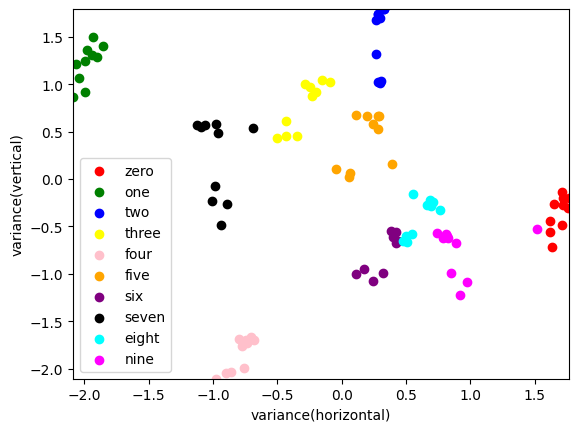
\includegraphics[width=0.8\textwidth]{image/vx_vy.png}
  \caption{横方向の分散と縦方向の分散}
  \label{fig:vx_vy}
\end{figure}

\begin{figure}[H]
  \centering
  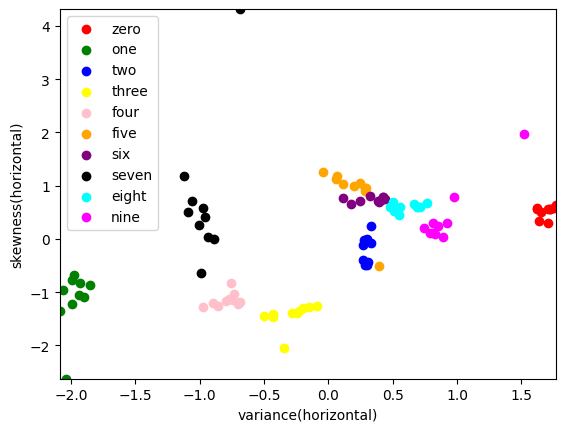
\includegraphics[width=0.8\textwidth]{image/vx_sx.png}
  \caption{横方向の分散と横方向のゆがみ}
  \label{fig:vx_sx}
\end{figure}

\begin{figure}[H]
  \centering
  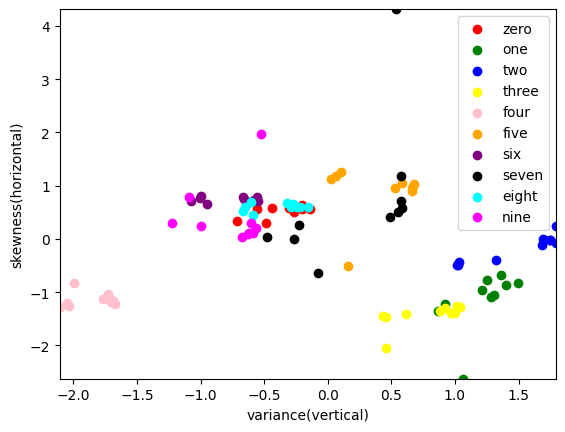
\includegraphics[width=0.8\textwidth]{image/vy_sx.png}
  \caption{縦方向の分散と横方向のゆがみ}
  \label{fig:vy_sx}
\end{figure}

\section{考察}
\subsection{特徴抽出}
表\ref{tab:csv}から分かるように,値の範囲がほぼ-2~2に収まっており,平均が0,分散が1となっているので,正規化と標準化が正しく行われていることが分かる.

\subsection{特徴評価}
特徴量の2次元組み合わせに関しては,結果のように求まったが,それらと図\ref{fig:vx_sx}~\ref{fig:vy_sx}を比較すると,評価値の大きいもの程まとまった分布をしていることが分かる.

\begin{thebibliography}{9}
  \item 崔恩瀞.プロジェクト実習Ⅱ パターン認識 実験テキスト.京都工芸繊維大学,2024年
\end{thebibliography}

\end{document}